\Chapter{Numerical Experiment}

Option Pricing has always been a challenging topic in financial mathematics. 
Although there are several other methods for pricing options, Monte Carlo performs better when solving high dimension problems.
In this chapter we makes several tests our reliable QMC with CV algorithm with option pricing problems. 
Note all our experiments are implemented under brownian motion (GBM) pricing model on non dividend paying stock.  
Since the GBM model is a well known model for option pricing, we only lay out the parameters for option formulas we use later and not dig into the model itself. 
\begin{align*}
    S(jT/d)&=\text{current asset price at time $jT/d,\; j=1,\dots,d$}\\
    K&=\text{strike price}\\
    T&=\text{expiration time}\\
    \sigma&=\text{volatility}\\
    r&=\text{interest rate}\\
    d&=\text{number of time steps}.
\end{align*}

\Section{Accuracy}

The first thing we want to test is whether our algorithm provides the `accurate' solution. This means if the function satisfies the cone condition, the difference between our estimation and true value should be bounded by the pre-defined error tolerance. We will test our algorithm for accuracy in three cases: without CV, single CV and multiply CV. 

To do this we have to know the exact value of our integral to calculate the exact error of our results. 
Therefore, we choose geomatric mean Asian option as our target function because they have exact solution for it under GBM model. We choose to test call options, so for geomatric mean Asian call option the payoff function is:   
\[ C_{T}^{\mathrm{gmean}} = \max\Big(\Big[\prod_{j=1}^{d}S(jT/d) \Big]^\frac{1}{d}-K, 0\Big)e^{-rT}.\]
The closed formula for exact price of it under GBM model is: 
\begin{align}
    C_{T}^{\mathrm{gmeanExact}} 
    &= S(0)e^{-(r+\sigma^2/2)T/2}\Phi(\tilde{d}_1)+Ke^{-rT}\Phi(\tilde{d}_2)    \label{eq:exactgmean}\\
    \tilde{d}_1 &=\frac{\ln(S(0)/K)+(r+\frac{n-1}{6(n+1)}\sigma^2/2)T/2}
    {\sqrt{\frac{2n+1}{6(n+1)}}\sigma\sqrt{T}}\notag\\
    \tilde{d}_2 &=\frac{\ln(S(0)/K)+(r-\sigma^2/2)T/2}
            {\sqrt{\frac{2n+1}{6(n+1)}}\sigma\sqrt{T}}\notag.
\end{align}

Then we need a couple control variates of which the exact solution must have clear formulas. 
Here we pick European call option and stock price at expiration as control variates.   
For European call option, the payoff function is: 
\[ C_{T} = \max (S(T)-K,0)e^{-rT}.\] 
The exact price of it under GBM model is given by:  
\begin{align*}
    C_{T}^{\mathrm{euroExact}} &= S(0)\Phi(d_1)-Ke^{-rT}\Phi(d_2)\\
    d_1 &=\frac{\ln(S_0/K)+(r+\sigma^2/2)T}{\sigma\sqrt{T}}\\
    d_2 &=\frac{\ln(S_0/K)+(r-\sigma^2/2)T}{\sigma\sqrt{T}}.
\end{align*}
For stock price, the payoff function is: 
\[ C_{T} = S(T)e^{-rT},\] 
while exact price of it under GBM model is just $S(0)$.  

The following is the set up for all options in the accuracy test:
\begin{table}[h]
    \centering
	\caption{Parameter Setup for accuracy test}
	\begin{tabular}{lllll}
		\hline\hline
        S0 & K & TimeVector & r & volatility \\[0.5ex]
        \hline
        120  & 100 & 1/52:1/52:4/52 & 0.01 & 0.5 \\[1ex] 
        \hline
	\end{tabular}
\end{table}.
We use in the money call option for both Asian and European options. 
They are monitored weekly for one month period with 1\% interest and 50\% volatility anunally. 

The test is then perform with three different absolute error tolerances as shown in table~\ref{tb:accuracy}.
First we caculated the exact price for the geomatric mean Asian call option using formula~\eqref{eq:exactgmean}. 
Then we run the same parameters through our reliable QMC algorithm to get the estimates. 
Finally we caluate the absolute value of difference between estimates and true prices as errors. 
We used three different absolute error tolerance set ups for this: $10^{-2}, 10^{-3}, 10^{-6}$.   
From the results we can see all errors lied within the preset tolerance. This give us confidence that our algorithm is at least accurate as guranteed.Note for second test, which the tolerance is $10^{-3}$, while the error seems all within a lesser bound $10^{-4}$. We believe this is not a error for the algorithm or the code.  It happened since each iteration our sample size is doubled and this could be more than satisfied for the predefined tolerance level.
\begin{table}[h]
    \label{tb:accuracy}
    \centering
	\caption{Accuracy Test of reliable QMC algorithm}
    \begin{tabular}{lrrr}  
    \hline \hline
    abstol = $10^{-2}$ & no CV&single CV&double CV\\[0.5ex]
    \hline
    exact price& 1.2926641930& 1.2926641930&1.2926641930\\[0.5ex]
    estimate price& 1.2938177355& 1.2937890386&1.2930809161\\[0.5ex]
    err=$|$exact-estimate$|$ & 1.1535e-3& 1.124e-3&4.167e-4\\[0.5ex]
    \hline
    abstol = $10^{-3}$ & no CV&single CV&double CV\\[0.5ex]
    \hline
    exact price& 1.2926641930& 1.2926641930&1.2926641930\\[0.5ex]
    estimate price& 1.2926529108& 1.2925687148&1.2925793049\\[0.5ex]
    err=$|$exact-estimate$|$ & 1.12821e-5& 9.54782e-5&8.48881e-5\\[0.5ex]
    \hline
    abstol = $10^{-6}$ & no CV&single CV&double CV\\[0.5ex]
    \hline
    exact price& 1.2926641930& 1.2926641930&1.2926641930\\[0.5ex]
    estimate price& 1.2926643000& 1.2926639635&1.296646297\\[0.5ex]
    err=$|$exact-estimate$|$ & 1.07e-7& 2.295e-7&4.367e-7\\[0.5ex]
    \hline
    \end{tabular}
\end{table}



\Section{Efficiency}

Now that we know our algorithm provides the desired results, we will go on test the time efficiency of our algorithm. 
Here we can not talk about time complexity using big O notation for the results depend not only on dimention but also  on target function itself. 
Instead, we do experiments to test the `efficiency' of our algorithm by compare the sample size used for caculation and the corresponding time cost. 
This test breaks into two parts.  
The first one is that we want to know how our algorithm performs without using control variates. Naturally the cubature sobol algorithm \cite{hickernell2014reliable} become a good reference. 
We know our algorithm is a bit slower compared to it when not using control variates. The question is how small the gap is. 
If there is no significant difference, then it means we will not waste too much time on cases without control variates or with poor control variates. 
The second one, which is more important, is that we want to see how much time it can save for using good control variates. Of course this depends on quality of the control variates. Fortunately, several good CV is known to be use for option pricing under GBM model \cite{lidebrandt2007variance}.         

\Subsection{reliable QMC without CV}
Parameter set up for efficiency test is shown in table\ref{tb:effsetup}. This time we try to price a weekly monitored 1-year period option, which increases the dimension to 52. Note we will keep using this set up for all the folloing efficienty tests. 
\begin{table}[h]
    \centering
    \label{tb:effsetup}
	\caption{Parameter Setup for efficienty test}
	\begin{tabular}{lllllll}
		\hline\hline
        S0 & K & TimeVector & r & volatility & abstol & reltol \\[0.5ex]
        \hline
        120  & 130 & 1/52:1/52:52/52 & 0.01 & 0.5 & 1e-3 & 0\\[1ex] 
        \hline
	\end{tabular}
\end{table}
We test our algorithm through four scenarors: the original adpaptive QMC,  our QMC\_CV without CV, QMC\_CV with single poor CV and QMC\_CV with two poor CV. 
For target option we still use geomtric mean Asian option European option. For single CV we use European option and add stock price for double CV. 
\begin{table}[h]
    \centering
    \label{tb:efftest1}
	\caption{Efficiency test I of reliable QMC algorithm}
    \begin{tabular}{rrrr}  
    \hline\hline
	\multicolumn{2}{c}{Sample Size}
		&\multicolumn{2}{c}{Time Cost} \\
    \hline
	 cubSobol&cubSobolcv
    &cubSobol&cubSobolcv\\[0.5ex]
    \hline
		 65535&9011
    &0.2783&0.0673\\[1ex]
    \hline
	\end{tabular}
\end{table}
As shown in table \ref{tb:efftest1}


\Subsection{reliable QMC with CV}
There are two types of asian options, depends on which types of mean one use. 
In last section we introduced geomatric mean Asian option, this time we choose arithematic mean asian call option as our target function, whose payoff function is:
\[ C_{T}^{Amean} = \max\Big(\frac{1}{d}\sum_{j=1}^{d}S(jT/d)-K, 0\Big)e^{-rT}.\]
For this option there is no close formula for exact price under GBM model.
However, recall we introduced another Asian option earlier of which the price has a clear formula. 
It is known that geomatric mean Asian option was first used as a CV for pricing arithmatic mean Asian option\cite{kemna1990pricing}.  
We start with this pair for efficiency test part II.

\begin{table}[h]
    \centering
    \label{tb:efftest2a}
	\caption{Efficiency test II of reliable QMC algorithm with Asian Option}
    \begin{tabular}{rrrr}  
    \hline\hline
	\multicolumn{2}{c}{Sample Size}
		&\multicolumn{2}{c}{Time Cost} \\
    \hline
	 cubSobol&cubSobolcv
    &cubSobol&cubSobolcv\\[0.5ex]
    \hline
		 65535&9011
    &0.2783&0.0673\\[1ex]
    \hline
	\end{tabular}
\end{table}

%Figure ~\ref{fg:cvEX1} shows decrease rate the walsh coefficients for the target function and control variates in this example.

\begin{figure}[h]
    \centering
    %\setlength{\unitlength}{0.14in}     % selecting unit length
    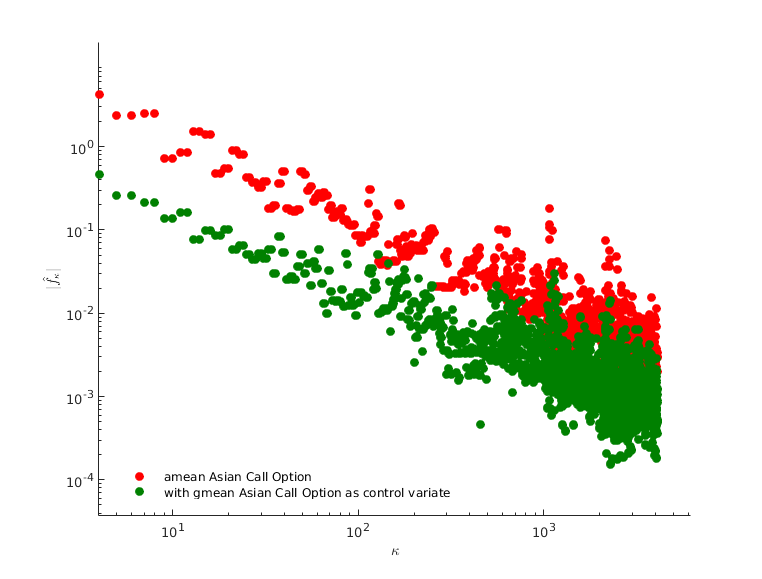
\includegraphics[width=\textwidth]{figures/cvEx1.eps}
    \label{fg:cvEX1}
    \caption{Walsh coefficients of $f$}
\end{figure}

\Subsection{Barrier Option}
Another good example is barrier option. This is the payoff function for up and in barrier call option:
\[ C_{T}^{\mathrm{U\&I}} = (S(T)-K)^+1_{ \{\max{S(jT/d)}\geq \mathrm{Barrier}\}}.\]
The reason we choose it is because of its similaritis to the European option. 
Note if the barrier equals strike price, then it is just an European call option, which makes european option a good control variates. 
For this test we take three different barriers which gradually grow further from the strick price. 
As same from last test, we compared oringinal reliable QMC algorithm and our CV version on sample size and time cost. 
\begin{table}[h]
    \centering
    \label{tb:}
	\caption{Results of cubSobol, cv\_old and cv\_new with Barrier Option}
    \begin{tabular}{lrrrr}
    \hline\hline
	Barrier &\multicolumn{2}{c}{Sample Size}
		&\multicolumn{2}{c}{Time Cost} \\
    \hline
	&no CV&with CV
    &no CV&with CV\\[0.5ex]
    \hline
	140  & 524288& 65535
	     & 1.874&0.2743 \\ 
	135  & 524288&6963
	     & 1.959&0.0519 \\ 
	130  & 524288&1024
    & 1.876& 0.0199 \\[1ex]
    \hline
	\end{tabular}
\end{table}
We can see from the results in table~\ref{tb:BarrierResults} that CV method takes nearly \% time lesser than.
